\documentclass[runningheads,a4paper]{llncs}
\usepackage{fontspec}
\setmainfont{cmunrm.otf}[BoldFont=cmunbx.otf,ItalicFont=cmunti.otf,BoldItalicFont=cmunbi.otf]
\setsansfont{cmunss.otf}[BoldFont=cmunsx.otf]
\setmonofont{cmuntt.otf}
\usepackage{microtype,graphicx,booktabs,tabularx,array,amsmath,amssymb,xcolor}
\usepackage{hyperref}
\newcolumntype{L}{>{\raggedright\arraybackslash}X}
\graphicspath{{figures/}}
\hypersetup{hidelinks,pdftitle={Deep Re-annotation and Controlled Candidate Pools for Re-evaluating Ranking Models on MS MARCO},pdfauthor={, , }}
\setlength{\emergencystretch}{1.5em}
\setlength{\tabcolsep}{4pt}
\renewcommand{\arraystretch}{1.12}
% Generated by build_tables.py from evaluation summaries.
\newcommand{\ManualQueryCount}{1\,179}
\newcommand{\ManualPairCount}{33\,667}
\newcommand{\FullQueryCount}{101\,093}
\newcommand{\JudgeTestAuc}{0.907}
\newcommand{\JudgeTestFOne}{0.875}
\newcommand{\JudgeTestPrecision}{0.851}
\newcommand{\JudgeTestRecall}{0.902}
\newcommand{\JudgeHeldoutOriginalNdcg}{0.512}
\newcommand{\JudgeHeldoutHumanNdcg}{0.938}
\newcommand{\FullPositiveLargeConditional}{130.70}
\newcommand{\OriginalPositiveCount}{1\,243}
\newcommand{\OriginalMeanRel}{1.05}
\newcommand{\HumanPositiveCount}{20\,597}
\newcommand{\HumanMeanRel}{17.47}
\newcommand{\JudgePositiveCount}{22\,206}
\newcommand{\JudgeMeanRel}{18.83}
\newcommand{\BmOriginal}{0.248}
\newcommand{\BmHuman}{0.644}
\newcommand{\EOriginal}{0.488}
\newcommand{\EHuman}{0.879}
\newcommand{\FullPoolSmall}{21.88}
\newcommand{\FullPositiveSmall}{14.19}
\newcommand{\FullPoolLarge}{451.54}
\newcommand{\FullPositiveLarge}{128.64}

\title{Deep Re-annotation and Controlled Candidate Pools for Re-evaluating Ranking Models on MS MARCO}
\titlerunning{Deep Re-annotation and Controlled Candidate Pools}
\author{}
\authorrunning{}
\institute{}

\begin{document}
\maketitle
\begin{abstract}
Sparse relevance judgments can leave correct answers uncredited when retrieval systems are evaluated. We study additional manual annotation on English MS MARCO using \ManualQueryCount{} queries and \ManualPairCount{} pooled query--passage pairs. Here, deep re-annotation means judging multiple candidate answers within a defined pool, rather than assuming that the original positive passage exhausts the relevant answers. With unchanged rankings, the mean number of positive judgments increases from \OriginalMeanRel{} to \HumanMeanRel{} per query. Under a common pool-based normalization and the same query set, NDCG@10 increases from \BmOriginal{} to \BmHuman{} for BM25 and from \EOriginal{} to \EHuman{} for E5. A compact cross-encoder judge achieves held-out ROC-AUC \JudgeTestAuc{} and is used to generate pseudo-labels for \FullQueryCount{} queries. We recompute these labels from saved scores at a fixed threshold and analyze pooling depths from 10 to 200. Candidate selection changes both label coverage and the interpretation of rank-fusion results. The findings concern the evaluated pools and do not imply exhaustive relevance annotation of the corpus or generalization across search providers and user populations.
\keywords{Information retrieval \and MS MARCO \and relevance judgments \and re-annotation \and pooling \and reciprocal rank fusion}
\end{abstract}

\section{Introduction}
\label{sec:intro}

Information retrieval evaluation requires queries, documents, and judgments of which documents satisfy each query. MS MARCO is a widely used collection built from real Bing search queries \cite{bajaj2016msmarco}. Its passage-ranking task provides query and passage texts and sparse relevance judgments, commonly called \emph{qrels}, short for query relevance judgments \cite{msmarco_datasets}. Most queries in the labeled development subset have only one positive passage. Other acceptable answers may remain unjudged and therefore contribute no gain to the evaluation metric.

MS MARCO is one of several search-provider datasets, not a universal sample of information needs. Google's Natural Questions contains real search queries with human answer annotations on Wikipedia pages \cite{kwiatkowski2019naturalquestions}. Yahoo!'s Learning to Rank Challenge released two sets of query--document feature vectors and graded relevance labels without query or document text \cite{chapelle2011yahoo}. Yandex's Personalized Web Search Challenge released session and click logs with anonymized identifiers rather than readable queries and documents \cite{yandex2013personalized}. These are useful counterparts in search research, but their tasks and released representations differ from passage ranking.

We focus on MS MARCO because its accessible texts, sparse human judgments, established evaluation tools, and pretrained models support comparisons with prior work. The sparse judgments also provide a direct setting for studying additional annotation. This choice does not establish universality: provider-specific sampling, language, query intent, and document domain may affect transfer. Differences between countries or social groups are not measured in this study.

By \emph{deep re-annotation} we mean extending relevance judgments across the candidate documents in a defined pool. ``Deep'' refers to annotation coverage, not neural-network depth or repeated training. It does not mean that the entire corpus has been exhaustively judged. For example, a query about why a liquid's boiling point increases may have several passages explaining the addition of salt. If only one passage is in the original qrels, another correct explanation receives zero gain until it is judged. Section~\ref{sec:example} gives an actual example with passage identifiers and before/after labels.

The retrieval rankings are held fixed when comparing original and human labels. Thus, an increase in measured NDCG after annotation does not mean that a retrieval model itself has improved. It means that its existing output is evaluated against more complete judgments. A second part of the study uses a learned judge to extend label coverage to larger candidate pools. These predictions are called \emph{pseudo-labels} to distinguish them from human judgments.

We address three questions: (1) how does additional manual annotation change label coverage and measured ranking quality; (2) how well does a compact judge agree with held-out human labels; and (3) how do pooling depth and the input depth of Reciprocal Rank Fusion (RRF) \cite{cormack2009rrf} affect evaluation? The contribution is an analysis of annotation and evaluation choices, rather than a new retrieval architecture.

\section{Related Work}
\label{sec:related}

MS MARCO supports both training and evaluation of neural retrieval models \cite{bajaj2016msmarco}. The mMARCO dataset extends passage ranking to multiple languages through translation \cite{bonifacio2022mmarco}; its Russian portion also appears in RusBEIR \cite{2025rusbeir}. Our experiments use English query and passage texts. Beyond a single provider, BEIR evaluates retrieval across 18 datasets with different tasks and domains \cite{thakur2021beir}. Cross-dataset evaluation addresses transfer across collections, but does not by itself establish demographic representativeness.

BM25 is a lexical baseline based on term matching, term frequency, and document-length normalization \cite{robertson2009bm25}. Dense bi-encoders such as E5 and BGE represent a query and a document separately and compare their vectors \cite{wang2022e5,xiao2023cpack}. Cross-encoders instead process the query and candidate jointly, allowing token-level interactions at a higher computational cost \cite{nogueira2019bert}. These distinctions matter because different systems can contribute different relevant passages to a pool.

Pooling is a standard test-collection construction method: top-ranked documents from several sources are merged and assessed by humans \cite{voorhees2005trec}. It reduces annotation effort but makes label coverage depend on the contributing systems and depth. RRF combines input ranks without training a score-calibration model \cite{cormack2009rrf}. Its behavior can depend on truncation, the input systems, and fusion parameters \cite{bruch2023fusion}. Our evaluation therefore states both the candidate-pool definition and the rankings supplied to fusion.

\section{Data and Manual Re-annotation}
\label{sec:data}

\subsection{Source Collection and Candidate Pool}

The English MS MARCO passage corpus contains 8,841,823 passages. The official development qrels used here contain 7,437 positive pairs for 6,980 queries \cite{msmarco_datasets}. The manual subset contains \ManualQueryCount{} queries and \ManualPairCount{} distinct query--passage pairs, with 28.56 candidates per query on average and a maximum of 63. The larger pseudo-labeling experiment uses \FullQueryCount{} queries with saved ranked lists; this set is not identical to the 6,980-query labeled development subset.

The manual pool was assembled by combining query-based retrieval results with auxiliary candidate-selection channels. Each query has ten entries in the saved BM25, E5, and BGE rankings. The annotation data also retain the auxiliary channels named \texttt{e5-rerank} and \texttt{s0}--\texttt{s3}. They contribute candidates beyond the three query-only lists. In particular, 6,258 pairs have no score in BM25, E5, BGE, or \texttt{e5-rerank}; 35 pools contain more than 40 documents. Thus, the annotation pool includes additional candidates beyond the four named top-ten lists.

Candidate preparation also used E5-based similarity to a known relevant answer, as part of the reference-assisted annotation procedure. This signal has access to answer information unavailable to ordinary query-only retrieval. The full pool is retained for annotation analysis. The controlled ranking comparison uses BM25, E5, BGE, and their three-way RRF; auxiliary channels contribute to pooling but are excluded from system-level comparisons because their model provenance is not established. The full-set rankings use \texttt{intfloat/e5-small-v2} and \texttt{BAAI/bge-small-en-v1.5}. These identifiers describe the full-set runs; the exact configurations of the auxiliary manual-pool channels remain unspecified.

\subsection{What the Assessor Judged}
\label{sec:annotation}

For each selected pair, the assessor saw the query, the candidate passage, and the original relevant MS MARCO passage. The task was to decide whether the candidate answered the same information need. Showing the reference passage helped align the interpretation with the initial annotation; it did not require the candidate to reproduce the reference wording. Pooling followed by these additional judgments is the deep re-annotation studied here.

The annotation records distinguish a seed-positive category and newly positive documents. For the sparse baseline, we use the official development qrels directly, intersected with the stored pool, rather than infer original relevance from the annotation category. This produces \OriginalPositiveCount{} positive pairs. Fourteen seed-marked pairs absent from the official qrels remain part of the extended human labels, but are not counted as official positives.

Human-positive labels cover \HumanPositiveCount{} pairs. There are also 13,041 explicit negative assessments and 29 nonstandard category values whose meaning is not established. The latter are left unjudged: they receive no gain at their original ranking positions, rather than being presented as verified negative assessments. Five passage-text fields are empty. A sensitivity analysis excludes all 23 queries affected by nonstandard labels or empty texts. The remaining 1,156 queries preserve the ranking order and the main annotation effect (Section~\ref{sec:manual-results}).

\begin{table}[t]
\caption{Annotation coverage within the same manual candidate pool. Automatic predictions are not additional human assessments.}
\label{tab:annotation-data}
\centering\small
\begin{tabularx}{\textwidth}{@{}Lrrr@{}}
\toprule
Quantity & Original & Human & Judge \\
\midrule
Queries & 1\,179 & 1\,179 & 1\,179 \\
Candidate pairs & 33\,667 & 33\,667 & 33\,667 \\
Positive pairs & 1\,243 & 20\,597 & 22\,206 \\
Positives per query, mean & 1.05 & 17.47 & 18.83 \\
Positives per query, median & 1 & 17 & 19 \\
\bottomrule
\end{tabularx}
\end{table}


The number of queries does not increase during manual re-annotation. What changes is the number of positive judgments within the same pool: the mean rises from \OriginalMeanRel{} to \HumanMeanRel{}, and the median from 1 to 17. These values characterize selected candidate sets and are not estimates of the total number of relevant passages in the corpus.

\subsection{A Concrete Example}
\label{sec:example}

Table~\ref{tab:example} illustrates query 1086224, ``what causes boiling point to increase''. The original positive passage explains that adding salt raises the boiling point. A second passage gives the same relevant explanation using the term ``non-volatile solute'', but is absent from the sparse qrels. A passage reporting acetone's boiling temperature does not explain the requested cause and has a negative human judgment in this pool.

\begin{table}[t]
\caption{Example from the manual data. Passage descriptions are shortened paraphrases, not new judgments. ``Unjudged'' means absent from the original positive qrels.}
\label{tab:example}
\centering\small
\begin{tabularx}{\textwidth}{@{}l L l l@{}}
\toprule
Passage ID & Passage content & Original & Human \\
\midrule
7112148 & Adding salt to water increases its boiling point. & Relevant & Relevant \\
7399382 & Adding a non-volatile solute, such as salt, raises a solvent's boiling point. & Unjudged & Relevant \\
987600 & Reports the boiling temperature of acetone. & Unjudged & Not relevant \\
\bottomrule
\end{tabularx}
\end{table}

Consider a system that returns passage 7399382 first. The sparse evaluation gives this result zero gain, although the passage addresses the question. After manual assessment it contributes positive gain, while the system output stays unchanged. This example distinguishes missing judgments from incorrect retrieval and explains why several relevant passages per query matter. It illustrates the procedure, not the frequency of any particular error across the collection.

\section{Judge and Evaluation Protocol}
\label{sec:protocol}

\subsection{Purpose and Input of the Judge}
\label{sec:judge-method}

Exhaustive human assessment of tens of millions of selected pairs is impractical. The judge transfers the signal of the manual judgments to larger pools. BM25, E5, and BGE continue to generate the candidates; the judge assigns relevance scores to already selected pairs. Its agreement with human labels must therefore be established separately from retrieval effectiveness.

We use the compact \texttt{cross-encoder/ms-marco-MiniLM-L6-v2} model \cite{wang2020minilm,reimers2019sentencebert}.\footnote{\url{https://huggingface.co/cross-encoder/ms-marco-MiniLM-L6-v2}} It processes the query and candidate passage jointly, unlike the separate encodings used by E5 and BGE. Its input contains the two texts only: no retrieval embeddings, ranks, fusion scores, or known relevant answer are supplied. MiniLM was selected as a public, computationally feasible MS MARCO baseline, not as the strongest available relevance judge.

The original training experiment split all 1,179 queries into 825 training, 177 validation, and 177 test queries, comprising 23,543, 5,122, and 5,002 pairs. The split uses query-group shuffling with seed 42, so a query cannot appear in more than one subset. Fine-tuning used two epochs, batch size 16, maximum sequence length 512, and 100 warmup steps. That training run mapped categories 1 and 2 to positive and the remaining categories to zero; the 29 unresolved categories are a limitation of the inherited training labels. The current evaluation does not relabel them as human-confirmed negatives.

The threshold selected on validation is \(\tau=-0.2187178284\). The base model's recorded validation ROC-AUC is 0.865. We recompute agreement from the saved fine-tuned scores on the same split and regenerate pseudo-qrels consistently as
\begin{equation}
\hat y(q,d)=\mathbb{I}[s(q,d)\geq\tau].
\label{eq:judge}
\end{equation}
All pseudo-label counts and threshold diagnostics use Eq.~\ref{eq:judge} with the same validation-selected threshold.

\begin{figure}[t]
\centering
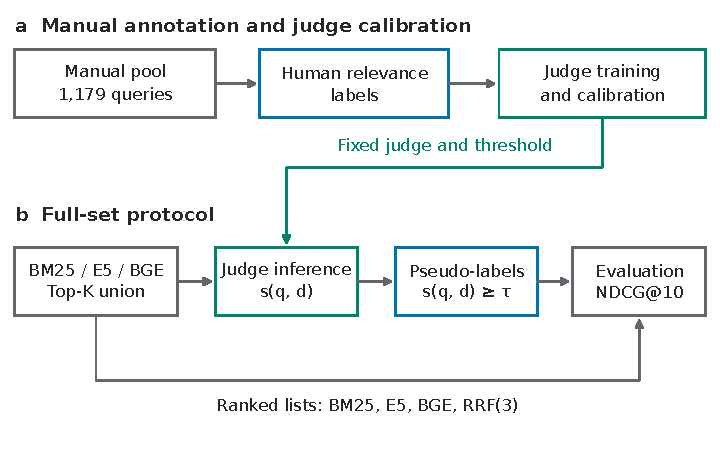
\includegraphics[width=\textwidth]{protocol_en.pdf}
\caption{The manual-annotation and automatic-labeling stages. Human labels supervise the judge; retrieval systems supply candidate passages.}
\label{fig:protocol}
\end{figure}

\subsection{Controlled Pools and Rank Fusion}
\label{sec:pool-method}

Let \(L_m(q)\) denote the saved ranking of system \(m\) for query \(q\). For the larger query set, the pool at depth \(K\) is
\begin{equation}
P_q^{(K)}=\bigcup_{m\in\{\mathrm{BM25,E5,BGE}\}}\mathrm{TopK}(L_m(q)),
\quad K\in\{10,30,50,100,200\}.
\label{eq:pool}
\end{equation}
Duplicates are removed by passage identifier. The judge's stored score is a property of the query--passage pair and is reused at every depth; enlarging the pool does not change that score. Pseudo-relevant passages are \(R_q^{(K)}=\{d\in P_q^{(K)}:\hat y(q,d)=1\}\).

Three-way fusion, denoted RRF(3), combines only BM25, E5, and BGE:
\begin{equation}
\mathrm{RRF}_K(d\mid q)=\sum_{m:d\in\mathrm{TopK}(L_m(q))}\frac{1}{60+\mathrm{rank}_m(d,q)}.
\label{eq:rrf}
\end{equation}
An absent document contributes zero for that input list. Ties are broken by ascending numeric passage identifier. In the manual experiment the available lists have depth ten. In the full-set experiment both pool depth and the input depth of \(\mathrm{RRF}_K\) vary. These are two distinct changes: the retrievers' own top-ten rankings remain fixed, whereas the fused top ten may change when deeper input lists are supplied. An additional analysis fixes fusion input at 200 while varying only the assessment pool.

\subsection{Metrics and Statistical Tests}
\label{sec:metrics}

NDCG@10 is normalized discounted cumulative gain at the first ten positions. With binary relevance, the numerator rewards relevant passages more strongly at earlier ranks. For a fixed pool and label set,
\begin{align}
\mathrm{DCG}@10(q,m)&=\sum_{i=1}^{10}\frac{y(q,L_m(q)_i)}{\log_2(i+1)},\\
\mathrm{IDCG}@10(q)&=\sum_{i=1}^{\min(10,|R_q|)}\frac{1}{\log_2(i+1)},\\
\mathrm{NDCG}@10(q,m)&=\frac{\mathrm{DCG}@10(q,m)}{\mathrm{IDCG}@10(q)}.
\label{eq:ndcg}
\end{align}
The ideal denominator is shared by all systems for that query and label set. It is computed from all positive judgments in the pool, not only from positives retrieved by the particular system. A query with no retrieved positives receives zero. If the pool has no positive judgments, its NDCG is defined as zero for every system. All reported system means use the same query set; no system-specific successful-query filter is applied. Unjudged passages retain their rank positions and contribute zero gain. These remain pool-based evaluations rather than full-corpus leaderboard scores.

Manual before/after comparisons use all 1,179 queries. We calculate paired query-level differences, 95\% percentile bootstrap intervals with 5,000 resamples, and two-sided paired sign-flip tests with 10,000 randomizations. The Monte Carlo estimate uses the correction \((b+1)/(B+1)\), where \(b\) is the number of randomized absolute effects at least as large as the observed effect. The four manual annotation-effect tests are also checked against a Bonferroni familywise level of 0.05. Full-set intervals use the resampling settings reported with Table~\ref{tab:fullset}; the query, rather than the individual passage, remains the resampling unit.

\section{Results of Manual Re-annotation}
\label{sec:manual-results}

Table~\ref{tab:manual-results} compares identical rankings under official sparse labels and additional human judgments. Every reported change is both a difference of means and a mean paired difference, because both columns contain the same 1,179 queries. The changes describe evaluation sensitivity to annotation coverage, not retraining of the retrieval models.

\begin{table}[t]
\caption{Pooled NDCG@10 before and after manual annotation on all 1,179 queries. These are not full-corpus leaderboard scores. $\Delta$ is human minus original; intervals are paired 95\% bootstrap intervals.}
\label{tab:manual-results}
\centering\small
\begin{tabularx}{\textwidth}{@{}Lrrrr@{}}
\toprule
System & Original & Human & $\Delta$ & 95\% CI \\
\midrule
BM25 & 0.248 & 0.644 & +0.396 & [0.372, 0.419] \\
E5 & 0.488 & 0.879 & +0.391 & [0.365, 0.417] \\
BGE & 0.433 & 0.828 & +0.395 & [0.369, 0.419] \\
RRF(3) & 0.459 & 0.854 & +0.395 & [0.371, 0.419] \\
\bottomrule
\end{tabularx}
\end{table}


All four mean changes are positive, their confidence intervals exclude zero, and the paired tests give \(p<0.001\), including the familywise correction. E5 has the highest human-label NDCG among the three query-only retrievers. RRF(3) lies between E5 and BGE; it does not improve on E5 in this manual setting. These comparisons concern the query-only retrievers and their fusion; the auxiliary annotation channels are outside the system-level comparison.

\begin{figure}[t]
\centering
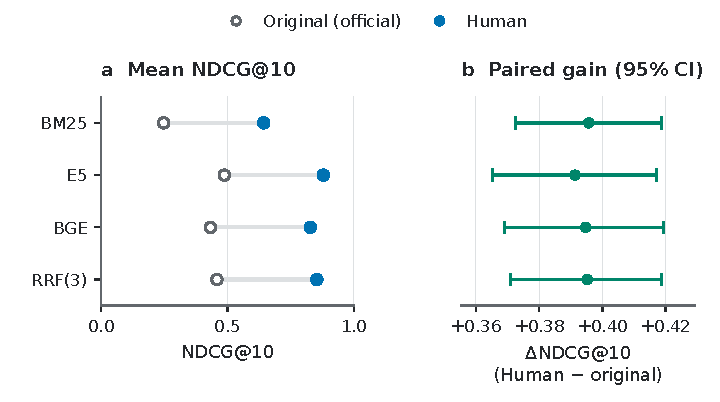
\includegraphics[width=\textwidth]{manual_effect_en.pdf}
\caption{Manual-pool evaluation on the same 1,179 queries with a shared ideal denominator. The paired effect intervals reflect uncertainty across queries, not variation between independently trained models.}
\label{fig:manual-effect}
\end{figure}

Excluding the 23 queries with unresolved category values or missing passage text leaves 1,156 queries. Human-label NDCG remains 0.644 for BM25, 0.879 for E5, 0.828 for BGE, and 0.855 for RRF(3), with the same system order. This check limits the influence of those data-quality issues on the manual comparison, but it does not substitute for a new assessment of ambiguous labels or an inter-assessor agreement study.

\subsection{Judge Agreement and Its Interpretation}
\label{sec:judge-results}

Table~\ref{tab:judge-results} separates the recorded base-model validation result from agreement recomputed using the saved fine-tuned scores. On the held-out test queries, the fine-tuned judge has ROC-AUC \JudgeTestAuc{}, F1 \JudgeTestFOne{}, precision \JudgeTestPrecision{}, and recall \JudgeTestRecall{}. The threshold is held fixed after validation.

\begin{table}[t]
\caption{Judge agreement. The base validation AUC is the recorded training baseline; fine-tuned metrics are recomputed from saved scores. P: precision; R: recall.}
\label{tab:judge-results}
\centering\small
\begin{tabularx}{\textwidth}{@{}Lrrrrrr@{}}
\toprule
Model / subset & Queries & Pairs & AUC & F1 & P & R \\
\midrule
Base / validation & 177 & 5\,122 & 0.865 & -- & -- & -- \\
Fine-tuned / validation & 177 & 5\,122 & 0.908 & 0.868 & 0.829 & 0.912 \\
Fine-tuned / test & 177 & 5\,002 & 0.907 & 0.875 & 0.851 & 0.902 \\
\bottomrule
\end{tabularx}
\end{table}


As an additional check of its behavior under the original judgments, ranking the entire manual candidate pool by judge score on the 177 held-out queries gives NDCG@10 \JudgeHeldoutOriginalNdcg{} with official labels and \JudgeHeldoutHumanNdcg{} with human labels. This is conditional reranking of an already enriched pool. It is not the judge's first-stage retrieval performance on the full corpus, and does not establish that it is stronger than all candidate-generating systems.

\begin{figure}[t]
\centering
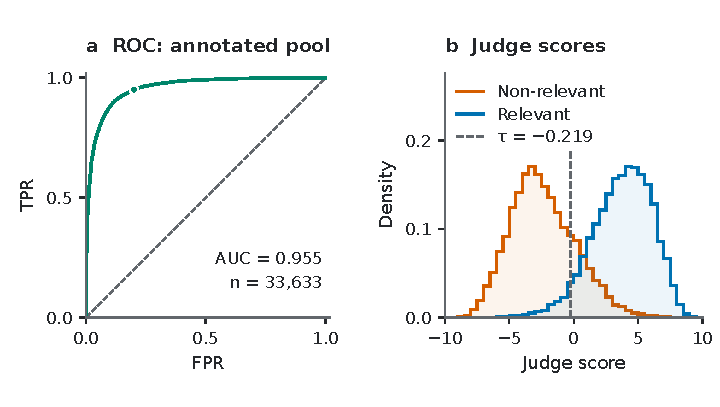
\includegraphics[width=\textwidth]{judge_diagnostics_en.pdf}
\caption{Score diagnostics on manual pairs with standard labels and nonempty text. This pool includes training queries; the figure is not an independent test-set estimate. Held-out agreement is reported separately in Table~\ref{tab:judge-results}.}
\label{fig:judge}
\end{figure}

Applying Eq.~\ref{eq:judge} to all saved manual-pool scores yields \JudgePositiveCount{} pseudo-positive pairs, or \JudgeMeanRel{} per query, versus \HumanPositiveCount{} human positives. A larger number of predictions is not evidence of more accurate annotation: false positives and false negatives must both be considered. Human labels remain the basis for assessing judge quality; pseudo-labels are an experimental instrument for the larger pool study.

\section{Full-set Pseudo-labeling and Pool Depth}
\label{sec:fullset}

The full-set analysis regenerates labels from stored query--passage scores with the same threshold at every depth. Table~\ref{tab:fullset} reports candidate coverage, positive-label counts, and ranking metrics on a common query set. At depth ten there are \FullPoolSmall{} candidates and \FullPositiveSmall{} pseudo-positive passages per query on average. At depth 200 the corresponding values are \FullPoolLarge{} and \FullPositiveLarge{}.

\begin{table}[t]
\caption{Full-set pseudo-label evaluation on all 101,093 queries, including zero-positive pools. Pool and positive counts are means per query; system columns are NDCG@10. RRF input depth equals $K$. Paired intervals and tests use 2,000 query resamples/randomizations, seed 20260914.}
\label{tab:fullset}
\centering\small
\begin{tabularx}{\textwidth}{@{}Lrrrrrr@{}}
\toprule
$K$ & Pool & Positive & BM25 & E5 & BGE & RRF(3) \\
\midrule
10 & 21.88 & 14.19 & 0.649 & 0.871 & 0.851 & 0.852 \\
30 & 65.85 & 33.71 & 0.638 & 0.851 & 0.832 & 0.862 \\
50 & 110.36 & 49.42 & 0.635 & 0.847 & 0.829 & 0.856 \\
100 & 222.91 & 81.02 & 0.633 & 0.844 & 0.825 & 0.851 \\
200 & 451.54 & 128.64 & 0.632 & 0.842 & 0.824 & 0.850 \\
\bottomrule
\end{tabularx}
\end{table}


RRF(3) is below E5 at $K=10$ (0.852 versus 0.871), but above it at all four larger tested depths. At $K=200$, the paired difference is $+0.0088$, with 95\% CI $[0.0082, 0.0095]$. All five depth-specific contrasts have unadjusted paired $p<0.001$; they also pass a Bonferroni correction for these five comparisons at level 0.05. This is agreement with the fixed judge, not independently established human relevance superiority.

The individual retrievers' top-ten DCG values stay constant as $K$ grows: only their shared ideal denominator changes. In contrast, deeper RRF inputs can change the fused ranking itself. Keeping fusion input fixed at 200 gives NDCG 0.805 at assessment depth ten and 0.850 at depth 200. At depth ten, 145\,643 of its returned query--passage pairs lie outside the assessed pool and receive zero gain. This diagnostic separates missing judgments from the effect of truncating fusion inputs.

All 1,179 manual queries occur in the full set, so the full-set analysis is not a wholly independent held-out evaluation. Excluding them leaves 99\,914 queries. At depth 200 the RRF-minus-E5 difference is still $+0.0088$ (95\% CI $[0.0080, 0.0094]$), and the direction of all five depth comparisons is unchanged. The score audit covers all 45\,647\,587 candidate pairs with no missing scores; 1\,592 queries have no positive prediction at depth 200.


\begin{figure}[t]
\centering
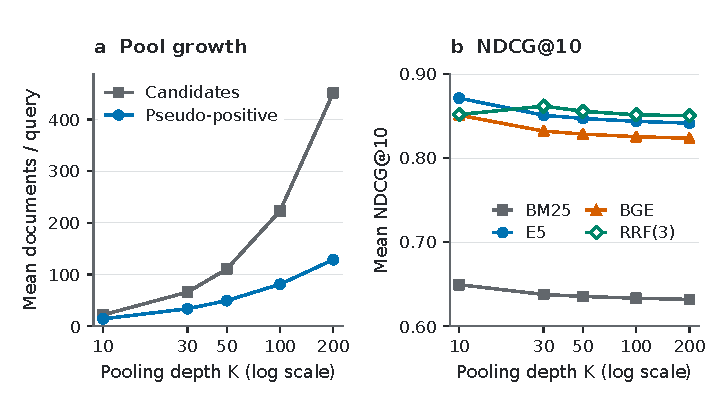
\includegraphics[width=\textwidth]{fullset_pooling_en.pdf}
\caption{Candidate coverage, pseudo-label density, and ranking behavior as pooling depth changes. All systems at a given depth share the same judgments and query set. RRF input truncation is distinguished from annotation-pool size.}
\label{fig:fullset}
\end{figure}

The conditional mean number of positives at depth 200 is \FullPositiveLargeConditional{} when queries without a positive prediction are excluded. The unconditional mean is \FullPositiveLarge{}. Both use the same total positive count but different denominators. Consequently, a statement such as ``about 130 relevant documents per query'' must specify the candidate pool, the judge, the threshold, and whether zero-positive queries are included. It is not an estimate of the true relevance density of the full corpus.

\section{Limitations and Discussion}
\label{sec:discussion}

\paragraph{Annotation and pooling.}
Human assessment covers selected candidates, not the whole corpus. The use of a known answer during candidate preparation and human judging enriches the pool and can anchor the interpretation of relevance. This helps find alternative answers but may underrepresent other valid interpretations of an ambiguous query. Exact attribution of every auxiliary channel and independent inter-assessor agreement are outside the controlled comparison. Nonstandard labels and empty texts are documented, and the query-exclusion sensitivity check does not remove all possible annotation errors.

\paragraph{Judge quality.}
MiniLM is a baseline cross-encoder. Its held-out agreement supports using it for a controlled score-based analysis, but its pseudo-labels are not human ground truth. Diagnostics that include training queries must not be confused with held-out estimates. The original training's handling of unresolved label categories is another limitation. Larger or more recent rerankers, including BGE cross-encoder variants, may produce different labels and system comparisons.

The automatic judge in this experiment receives a query and candidate only. This is a deliberately restricted baseline, not a requirement that an assessor must have the same information as a retrieval system. A known relevant answer can legitimately be provided to the judge without providing it to the retriever. A future reference-conditioned judge should therefore use ``query, known relevant answer, candidate passage'' and be evaluated against held-out human judgments. No comparison with such a model is claimed here.

\paragraph{Evaluation and transfer.}
Both the definition of IDCG and the treatment of zero-positive queries affect reported means. Pool expansion may change the available labels, while deeper RRF inputs may additionally change the ranking. The two effects should be reported separately. Pseudo-labeling also cannot establish that a model is universally better merely because it agrees more closely with this particular judge.

Our findings concern English MS MARCO and the evaluated pools. Provider, language, intent, and document-domain differences may change the results. Geographic or social-group transfer has not been tested, and no population representativeness is claimed. Evaluation on heterogeneous collections such as BEIR is a natural next step \cite{thakur2021beir}; multilingual translation alone would not establish demographic coverage.

\section{Conclusion}
\label{sec:conclusion}

Deep re-annotation in this study means increasing the coverage of human relevance judgments inside a defined candidate pool. On 1,179 queries, additional judgments increase the mean positive count from \OriginalMeanRel{} to \HumanMeanRel{}. Measured NDCG@10 rises for BM25, E5, BGE, and RRF(3) when the same rankings and query set are evaluated against these denser labels. E5 remains the best of the three query-only retrievers in the manual experiment.

The MiniLM judge enables a larger controlled pseudo-labeling analysis and reaches held-out ROC-AUC \JudgeTestAuc{}. Its input is intentionally restricted to query and candidate text. Future work should compare stronger cross-encoders and a judge conditioned on the known relevant answer, using the format ``query, known relevant answer, candidate passage''. Such a study would test the value of reference information for assessment rather than assume that the current baseline is optimal.

Candidate-pool depth is essential for interpreting the full-set results. RRF(3) is below E5 at input depth ten but above it at the four larger tested depths under the judge's labels. Positive-label counts depend on which documents are scored, and rank fusion also depends on the depth of its input lists. Neither a high pseudo-positive count nor a fusion advantage can be transferred to another evaluation setting without checking these conditions.

In practical terms, additional annotation and automatic pseudo-labeling are useful research instruments when the candidate selection, normalization, threshold, and evaluation population are explicit. Re-evaluating MS MARCO therefore concerns both improving judgment coverage and defining a consistent measurement procedure, with transfer beyond this collection left to further empirical validation.

\begin{thebibliography}{99}
\bibitem{bajaj2016msmarco}
Bajaj, P., Campos, D., Craswell, N., et al.: MS MARCO: A Human Generated MAchine Reading COmprehension Dataset. arXiv:1611.09268 (2016).
\url{https://arxiv.org/abs/1611.09268}

\bibitem{msmarco_datasets}
Microsoft: MS MARCO datasets and passage-ranking resources.
\url{https://microsoft.github.io/msmarco/Datasets}. Accessed 14 September 2026.

\bibitem{kwiatkowski2019naturalquestions}
Kwiatkowski, T., Palomaki, J., Redfield, O., et al.: Natural Questions: A Benchmark for Question Answering Research. Transactions of the Association for Computational Linguistics 7 (2019).
\url{https://doi.org/10.1162/tacl_a_00276}

\bibitem{chapelle2011yahoo}
Chapelle, O., Chang, Y.: Yahoo! Learning to Rank Challenge Overview. In: Proceedings of the Learning to Rank Challenge. PMLR 14, pp. 1--24 (2011).
\url{https://proceedings.mlr.press/v14/chapelle11a.html}

\bibitem{yandex2013personalized}
Yandex: Personalized Web Search Challenge. Kaggle competition (2013--2014).
\url{https://www.kaggle.com/c/yandex-personalized-web-search-challenge}.
Accessed 14 September 2026.

\bibitem{bonifacio2022mmarco}
Bonifacio, L., Jeronymo, V., Abonizio, H.Q., Campiotti, I., Fadaee, M., Lotufo, R., Nogueira, R.: mMARCO: A Multilingual Version of MS MARCO Passage Ranking Dataset. arXiv:2108.13897 (2021).
\url{https://arxiv.org/abs/2108.13897}

\bibitem{2025rusbeir}
Building Russian Benchmark for Evaluation of Information Retrieval Models. Computational Linguistics and Intellectual Technologies (2025).
\url{https://arxiv.org/abs/2504.12879}

\bibitem{thakur2021beir}
Thakur, N., Reimers, N., R\"uckl\'e, A., Srivastava, A., Gurevych, I.: BEIR: A Heterogeneous Benchmark for Zero-shot Evaluation of Information Retrieval Models. Proceedings of the Neural Information Processing Systems Track on Datasets and Benchmarks 1 (2021).
\url{https://arxiv.org/abs/2104.08663}

\bibitem{robertson2009bm25}
Robertson, S.E., Zaragoza, H.: The Probabilistic Relevance Framework: BM25 and Beyond. Foundations and Trends in Information Retrieval 3(4), 333--389 (2009).

\bibitem{wang2022e5}
Wang, L., Yang, N., Huang, X., Jiao, B., Yang, L., Jiang, D., Majumder, R., Wei, F.: Text Embeddings by Weakly-Supervised Contrastive Pre-training. arXiv:2212.03533 (2022).
\url{https://arxiv.org/abs/2212.03533}

\bibitem{xiao2023cpack}
Xiao, S., Liu, Z., Zhang, P., Muennighoff, N., Lian, D., Nie, J.-Y.: C-Pack: Packed Resources for General Chinese Embeddings. arXiv:2309.07597 (2023).
\url{https://arxiv.org/abs/2309.07597}

\bibitem{nogueira2019bert}
Nogueira, R., Cho, K.: Passage Re-ranking with BERT. arXiv:1901.04085 (2019).
\url{https://arxiv.org/abs/1901.04085}

\bibitem{cormack2009rrf}
Cormack, G.V., Clarke, C.L.A., B\"uttcher, S.: Reciprocal Rank Fusion outperforms Condorcet and Individual Rank Learning Methods. In: Proceedings of SIGIR, pp. 758--759 (2009).

\bibitem{bruch2023fusion}
Bruch, S., Gai, S., Ingber, A.: An Analysis of Fusion Functions for Hybrid Retrieval. arXiv:2210.11934 (2022; revised 2023).
\url{https://arxiv.org/abs/2210.11934}

\bibitem{voorhees2005trec}
Voorhees, E.M., Harman, D.K. (eds.): TREC: Experiment and Evaluation in Information Retrieval. MIT Press (2005).

\bibitem{wang2020minilm}
Wang, W., Wei, F., Dong, L., Bao, H., Yang, N., Zhou, M.: MiniLM: Deep Self-Attention Distillation for Task-Agnostic Compression of Pre-Trained Transformers. Advances in Neural Information Processing Systems 33, 5776--5788 (2020).

\bibitem{reimers2019sentencebert}
Reimers, N., Gurevych, I.: Sentence-BERT: Sentence Embeddings using Siamese BERT-Networks. In: Proceedings of EMNLP-IJCNLP, pp. 3982--3992 (2019).
\url{https://doi.org/10.18653/v1/D19-1410}
\end{thebibliography}

\clearpage
\section*{Reviewers' Remarks and Authors' Responses}
\label{sec:responses}
\noindent Submission 90. Revised for DAMDID 2026, 14 September 2026.

\paragraph{Reviewer 1: terminology and examples (weak accept).}
\emph{Remark, summarized and translated from Russian.} The paper has the necessary research sections, but the meaning of deep re-annotation is insufficiently clear. The reviewer asks for concrete examples and explanations that make the main concepts accessible to readers who are less familiar with the topic.

\emph{Response.} We have defined deep re-annotation operationally in the Introduction and Section~\ref{sec:annotation}: it means extending human judgments over a selected pool, not increasing neural-network depth or judging the entire corpus. Section~\ref{sec:example} and Table~\ref{tab:example} now give an actual MS MARCO query, passage identifiers, shortened passage descriptions, and before/after relevance status. The surrounding explanation shows why a correct but unjudged answer receives no gain under sparse qrels. We explicitly distinguish changes in measured quality from improvements to the unchanged retrieval models, and explain qrels, pooling, pseudo-labels, and the judge's input. These clarifications are also included in the Russian version.

\paragraph{Reviewer 2: overall assessment (accept).}
\emph{Remark, summarized.} The reviewer considers the dataset-improvement problem important, the results valuable, and the strategy justified, and supports publication as a full paper.

\emph{Response.} We thank the reviewer for this positive assessment. No specific additional change was requested. The revised article retains the focus on relevance-judgment coverage and adds the explanations and methodological clarifications described in this response.

\paragraph{Reviewer 3: other providers and universality (strong accept).}
\emph{Remark, summarized.} Are counterparts of MS MARCO available from Google, Yandex, or Yahoo? How universal is MS MARCO given possible differences in search-engine use between countries and social groups? The reviewer suggests explaining the choice of MS MARCO in the Introduction.

\emph{Response.} Section~\ref{sec:intro} now discusses Google's Natural Questions, Yahoo!'s Learning to Rank Challenge, and Yandex's Personalized Web Search Challenge with primary-source references. We distinguish text-based question answering, feature-based ranking, and anonymized interaction logs, rather than treat them as interchangeable datasets. We explain the choice of MS MARCO through available texts, sparse judgments, established tools, and pretrained models. Sections~\ref{sec:related} and \ref{sec:discussion} discuss cross-dataset evaluation and explicitly state that transfer across countries or social groups was not evaluated. The article makes no claim of demographic representativeness or universal validity.

\paragraph{Additional methodological corrections in this revision.}
During verification we found that the previous calculation used a system-specific ideal denominator and omitted queries without a retrieved positive. We have replaced it with a common pool-based IDCG and a common query population, and recomputed the ranking tables, paired effects, confidence intervals, and figures. The baseline now uses official development qrels directly, yielding 1,243 positive pairs in the manual pool; the median human-positive count is corrected to 17. Pseudo-labels are regenerated consistently from raw scores and the saved threshold, yielding 22,206 positives in the manual pool. We also make the auxiliary pooling channels explicit, restrict RRF to the three named query-only retrievers, and distinguish fusion-input depth from assessment-pool depth. These changes affect numerical values and delimit the conclusions; they are reported transparently rather than presented as purely editorial amendments. The qualitative finding that additional manual judgments increase measured NDCG remains supported under the revised protocol.

The full-set fusion comparison changes direction relative to the previous version: reconstructed RRF(3) is below E5 at depth ten and above it at the four larger tested depths. This result also holds after excluding all manual queries. Section~\ref{sec:fullset} and the Conclusion have been revised accordingly; we do not retain the previous claim about fusion behavior.

\end{document}
